\documentclass{article}
\usepackage{tikz}
\usepackage{amsmath}
\usepackage{amssymb}
\usepackage[utf8]{inputenc}
\usepackage{xcolor}
\usepackage{listings}

\usetikzlibrary{positioning, arrows.meta, shapes, calc}

\begin{document}

\begin{figure}[htbp]
\centering
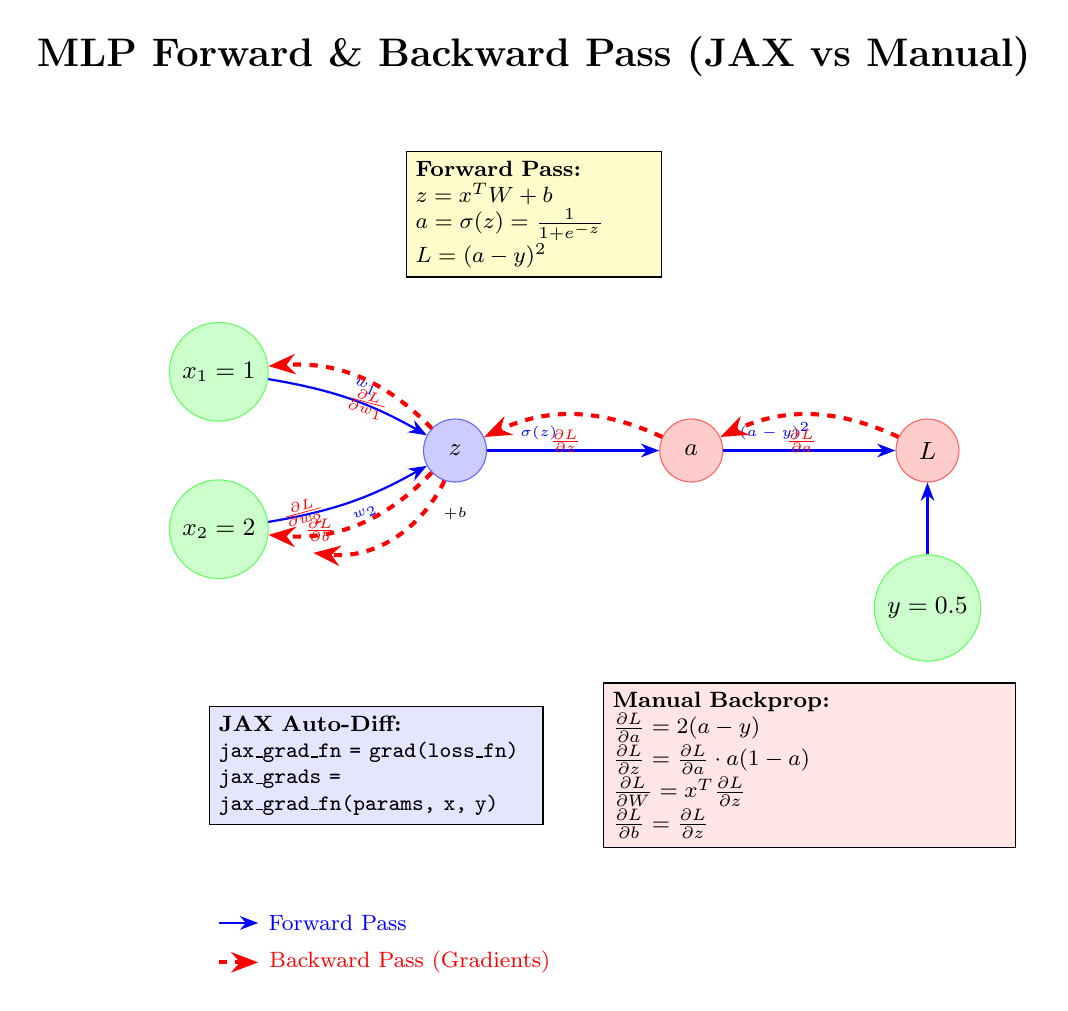
\begin{tikzpicture}[
    node distance=1.5cm,
    neuron/.style={circle, draw=blue!60, fill=blue!20, minimum size=0.8cm},
    input/.style={circle, draw=green!60, fill=green!20, minimum size=0.6cm},
    output/.style={circle, draw=red!60, fill=red!20, minimum size=0.8cm},
    arrow/.style={->, >=Stealth, thick},
    forward/.style={arrow, blue},
    backward/.style={arrow, red, dashed, line width=1.5pt},
    label/.style={font=\small}
]

% Title
\node[font=\Large\bfseries] at (0, 6) {MLP Forward \& Backward Pass (JAX vs Manual)};

% Input nodes
\node[input, label] (x1) at (-4, 2) {$x_1=1$};
\node[input, label] (x2) at (-4, 0) {$x_2=2$};

% Hidden layer (single neuron)
\node[neuron, label] (h1) at (-1, 1) {$z$};

% Activation
\node[output, label] (a1) at (2, 1) {$a$};

% Loss
\node[output, label] (loss) at (5, 1) {$L$};

% Target
\node[input, label] (target) at (5, -1) {$y=0.5$};

% Forward connections (with bend to avoid overlap)
\draw[forward] (x1) to[bend left=10] node[above left, sloped, font=\tiny, pos=0.7] {$w_1$} (h1);
\draw[forward] (x2) to[bend right=10] node[below left, sloped, font=\tiny, pos=0.7] {$w_2$} (h1);
\draw[forward] (h1) -- node[above, font=\tiny, pos=0.3] {$\sigma(z)$} (a1);
\draw[forward] (a1) -- node[above, font=\tiny, pos=0.3] {$(a-y)^2$} (loss);
\draw[forward] (target) -- (loss);

% Bias
\node[font=\tiny] at (-1, 0.2) {$+b$};

% Backward connections (gradients) - with more bend to clearly separate
\draw[backward] (loss) to[bend right=25] node[below right, font=\tiny, pos=0.7] {$\frac{\partial L}{\partial a}$} (a1);
\draw[backward] (a1) to[bend right=25] node[below right, font=\tiny, pos=0.7] {$\frac{\partial L}{\partial z}$} (h1);
\draw[backward] (h1) to[bend right=25] node[below right, sloped, font=\tiny, pos=0.6] {$\frac{\partial L}{\partial w_1}$} (x1);
\draw[backward] (h1) to[bend left=25] node[above left, sloped, font=\tiny, pos=0.6] {$\frac{\partial L}{\partial w_2}$} (x2);

% Additional bias gradient arrow
\draw[backward] (h1) to[bend left=35] node[above left, font=\tiny, pos=0.8] {$\frac{\partial L}{\partial b}$} (-2.8, -0.3);

% Equations box - JAX
\node[draw, fill=blue!10, text width=4cm, font=\footnotesize] at (-2, -3) {
\textbf{JAX Auto-Diff:} \\
\texttt{jax\_grad\_fn = grad(loss\_fn)} \\
\texttt{jax\_grads = jax\_grad\_fn(params, x, y)}
};

% Equations box - Manual
\node[draw, fill=red!10, text width=5cm, font=\footnotesize] at (3.5, -3) {
\textbf{Manual Backprop:} \\
$\frac{\partial L}{\partial a} = 2(a - y)$ \\
$\frac{\partial L}{\partial z} = \frac{\partial L}{\partial a} \cdot a(1-a)$ \\
$\frac{\partial L}{\partial W} = x^T \frac{\partial L}{\partial z}$ \\
$\frac{\partial L}{\partial b} = \frac{\partial L}{\partial z}$
};

% Forward pass equations
\node[draw, fill=yellow!20, text width=3cm, font=\footnotesize] at (0, 4) {
\textbf{Forward Pass:} \\
$z = x^T W + b$ \\
$a = \sigma(z) = \frac{1}{1+e^{-z}}$ \\
$L = (a - y)^2$
};

% Legend
\draw[forward] (-4, -5) -- (-3.5, -5) node[right, font=\footnotesize] {Forward Pass};
\draw[backward] (-4, -5.5) -- (-3.5, -5.5) node[right, font=\footnotesize] {Backward Pass (Gradients)};

\end{tikzpicture}
\caption{Forward and backward pass in a single-neuron MLP. JAX automatically computes gradients, while the manual method applies chain rule directly.}
\end{figure}

% Second figure: Computational Graph
\begin{figure}[htbp]
\centering
\begin{tikzpicture}[
    node distance=1cm,
    op/.style={rectangle, draw=black, fill=gray!20, minimum size=0.8cm},
    var/.style={ellipse, draw=blue, fill=blue!20, minimum width=1cm, minimum height=0.6cm},
    grad/.style={ellipse, draw=red, fill=red!20, minimum width=1cm, minimum height=0.6cm, dashed},
    arrow/.style={->, >=Stealth, thick}
]

\node[font=\Large\bfseries] at (0, 5) {Computational Graph};

% Variables
\node[var] (x) at (-4, 2) {$\mathbf{x}$};
\node[var] (W) at (-4, 0) {$\mathbf{W}$};
\node[var] (b) at (-4, -2) {$\mathbf{b}$};
\node[var] (y) at (4, -2) {$y$};

% Operations
\node[op] (matmul) at (-2, 1) {$\cdot$};
\node[op] (add) at (0, 0) {$+$};
\node[op] (sigmoid) at (2, 0) {$\sigma$};
\node[op] (sub) at (4, 0) {$-$};
\node[op] (square) at (6, 0) {$(\cdot)^2$};

% Forward edges - with slight curves to separate from backward
\draw[arrow, blue, line width=1.5pt] (x) to[bend left=8] (matmul);
\draw[arrow, blue, line width=1.5pt] (W) to[bend right=8] (matmul);
\draw[arrow, blue, line width=1.5pt] (matmul) to[bend left=8] (add);
\draw[arrow, blue, line width=1.5pt] (b) to[bend right=8] (add);
\draw[arrow, blue, line width=1.5pt] (add) to[bend left=8] (sigmoid);
\draw[arrow, blue, line width=1.5pt] (sigmoid) to[bend left=8] (sub);
\draw[arrow, blue, line width=1.5pt] (y) to[bend left=8] (sub);
\draw[arrow, blue, line width=1.5pt] (sub) to[bend left=8] (square);

% Intermediate variables - repositioned to avoid overlap
\node[var, font=\footnotesize] at (-2, 0.5) {$\mathbf{x^T W}$};
\node[var, font=\footnotesize] at (0, 0.8) {$z$};
\node[var, font=\footnotesize] at (2, 0.8) {$a$};
\node[var, font=\footnotesize] at (4, 0.8) {$a-y$};
\node[var, font=\footnotesize] at (6, 0.8) {$L$};

% Gradient nodes - repositioned with more spacing
\node[grad, font=\footnotesize] (gL) at (6, -2.8) {$\frac{\partial L}{\partial L}=1$};
\node[grad, font=\footnotesize] (ga_y) at (4, -3.8) {$\frac{\partial L}{\partial(a-y)}$};
\node[grad, font=\footnotesize] (ga) at (2, -3.8) {$\frac{\partial L}{\partial a}$};
\node[grad, font=\footnotesize] (gz) at (0, -3.8) {$\frac{\partial L}{\partial z}$};
\node[grad, font=\footnotesize] (gW) at (-2, -3.8) {$\frac{\partial L}{\partial W}$};
\node[grad, font=\footnotesize] (gb) at (-4, -4.5) {$\frac{\partial L}{\partial b}$};

% Backward edges - with curves to clearly separate from forward
\draw[arrow, red, dashed, line width=2pt] (gL) to[bend right=20] (ga_y);
\draw[arrow, red, dashed, line width=2pt] (ga_y) to[bend right=20] (ga);
\draw[arrow, red, dashed, line width=2pt] (ga) to[bend right=20] (gz);
\draw[arrow, red, dashed, line width=2pt] (gz) to[bend right=20] (gW);
\draw[arrow, red, dashed, line width=2pt] (gz) to[bend left=20] (gb);

% Comparison box
\node[draw, fill=green!10, text width=8cm, font=\footnotesize] at (1, -6.5) {
\textbf{Comparison Result:}
If the difference between JAX autodiff and manually computed gradients is $< 10^{-6}$, then ✅ Success!
\\
This demonstrates that JAX's automatic differentiation computes mathematically correct gradients.
};

\end{tikzpicture}
\caption{Automatic differentiation through computational graph. Forward pass (blue solid, thicker) computes values, backward pass (red dashed, thicker) propagates gradients.}
\end{figure}

\newpage

% Code section
\section*{JAX vs Manual Backpropagation Implementation}

% Configure listings for Python code with background
\lstset{
    language=Python,
    backgroundcolor=\color{gray!10},
    basicstyle=\ttfamily\footnotesize,
    breaklines=true,
    frame=single,
    rulecolor=\color{gray!30},
    showstringspaces=false,
    commentstyle=\color{green!60!black},
    keywordstyle=\color{blue!80!black},
    stringstyle=\color{red!60!black},
    numberstyle=\tiny\color{gray},
    captionpos=b
}

\begin{lstlisting}
import jax
import jax.numpy as jnp
from jax import grad

# 1. Define model parameters and data
# Fix random seed for reproducibility
key = jax.random.PRNGKey(0) 
key, w_key, b_key = jax.random.split(key, 3)

# MLP parameters (1 layer, 1 neuron)
W = jax.random.normal(w_key, (2, 1))  # Input dim 2, output dim 1
b = jax.random.normal(b_key, (1,))    # Bias
params = {'W': W, 'b': b}

# Sample data
x = jnp.array([1.0, 2.0])
y_true = jnp.array([0.5])  # Target value

# 2. Define MLP and loss function (Sigmoid activation)
def sigmoid(z):
    return 1 / (1 + jnp.exp(-z))

def mlp(params, x):
    # Linear transformation of input x
    z = jnp.dot(x, params['W']) + params['b']
    # Apply sigmoid activation function
    return sigmoid(z)

def loss_fn(params, x, y_true):
    y_pred = mlp(params, x)
    # L2 loss (Mean Squared Error)
    return jnp.mean((y_pred - y_true) ** 2)

# 3. Gradient calculation using JAX
jax_grad_fn = grad(loss_fn)
jax_grads = jax_grad_fn(params, x, y_true)

print("--- Gradients computed by JAX ---")
print("dW:", jax_grads['W'])
print("db:", jax_grads['b'])

# 4. From Scratch (manual) gradient calculation
# Apply backpropagation principles
def manual_grads(params, x, y_true):
    W, b = params['W'], params['b']

    # Forward propagation
    z = jnp.dot(x, W) + b
    a = sigmoid(z)
    loss = jnp.mean((a - y_true) ** 2)

    # Backward propagation - Chain rule
    # L2 loss derivative: dL/da = 2 * (a - y_true)
    grad_a = 2 * (a - y_true)

    # Sigmoid derivative: da/dz = a * (1 - a)
    # dL/dz = dL/da * da/dz = 2 * (a - y_true) * a * (1 - a)
    grad_z = grad_a * a * (1 - a)

    # z = x^T W + b derivatives
    # dL/dW = dL/dz * dz/dW = grad_z * x^T
    grad_W = jnp.outer(x, grad_z) 

    # dL/db = dL/dz * dz/db = grad_z * 1
    grad_b = grad_z
    
    return {'W': grad_W, 'b': grad_b}

manual_grads_dict = manual_grads(params, x, y_true)

print("\n--- Gradients computed from scratch ---")
print("dW:", manual_grads_dict['W'])
print("db:", manual_grads_dict['b'])

# 5. Compare results
print("\n--- Result comparison ---")
# Calculate error between the two gradients
dw_diff = jnp.sum(jnp.abs(jax_grads['W'] - manual_grads_dict['W']))
db_diff = jnp.sum(jnp.abs(jax_grads['b'] - manual_grads_dict['b']))

print(f"dW error: {dw_diff}")
print(f"db error: {db_diff}")

# If error is less than 1e-6, they are essentially identical
if dw_diff < 1e-6 and db_diff < 1e-6:
    print("✅ JAX and manual gradients are identical!")
else:
    print("❌ Gradients differ between methods.")
\end{lstlisting}

\end{document}